\documentclass{article}
\title{心理学入門 — 心のしくみはどう測られてきたか}
\author{TeX 図書館}

\begin{document}

\section{読み方 — この本の地図と 3 つの道具}

心理学は「心の counseling(相談)」ではありません。\textbf{心の働きを実験で測り、法則として記述する科学}です。見えない心をどうやって扱うのか。その答えが、この本を貫く 3 つの道具です。

\begin{enumerate}
\item \textbf{測る}: 心の働きを、反応時間・正答率・誤差といった数に変換する。
\item \textbf{比べる}: 条件を変えた 2 つの群を比べて、差が本当かを確かめる。
\item \textbf{再現する}: 同じ実験を別の人・別の時に繰り返して、結果が残るか確かめる。
\end{enumerate}

「心理学は当てずっぽう」という印象の正体は、この道具の不在です。逆に言えば、道具をそろえた話だけを受け取れば、心理学は極めて堅実な科学になります。この本では、有名な実験を必ず「どう測り、どう比べたか」まで遡って紹介します。

\subsection{全 10 節の見取り図}

節の配分は次のとおりです。

\begin{enumerate}
\item 第 1 節: 読み方。科学としての心の測り方。
\item 第 2 節: 知覚。見ることは解釈すること。
\item 第 3 節: 記憶。3 つの貯蔵庫と忘却の法則。
\item 第 4 節: 学習。条件づけと強化の仕組み。
\item 第 5 節: 発達。こころの成長の段階。
\item 第 6 節: 社会心理。人は場にどう動かされるか。
\item 第 7 節: 判断の近道。ヒューリスティックとバイアス。
\item 第 8 節: 感情とストレス。仕組みと対処。
\item 第 9 節: 性格。型で語る危険と次元で測る方法。
\item 第 10 節: まとめと次の一歩。
\end{enumerate}

各節の終わりには\textbf{解答の指針}を置きます。答えの丸写しではなく、「この実験の条件設定は何か」を自分の言葉で書く欄です。心理学の理解は、実験の構造が書けるかどうかで決まります。

\begin{quote}
\textbf{【注意】}\ 心理学の結論は「すべての人に必ず当てはまる」ものではありません。実験は平均的な傾向を示すだけで、個人差は常にあります。この本の記述はすべて「統計的な傾向」として読んでください。
\end{quote}

\textbf{解答の指針:}\ 有名な実験を学ぶときは、(1) 何を測ったか、(2) 何と何を比べたか、(3) 対照群(比べる基準)はどう作ったか、を自分の言葉で 1 行ずつ書く。結果の面白さに飛びつく前に、実験の構造を押さえるのが心理学の読み方です。

\section{知覚 — 見ることは解釈すること}

「目はカメラ」と思いがちですが、知覚の実験は違うことを示します。\textbf{目から入るのは不完全なデータで、脳がそれを解釈して「見えている世界」を作っている}のです。だから知覚は、物理的な刺激だけでなく、過去の経験や期待にも動かされます。

\subsection{錯視が教えてくれること}

有名なミュラー・リヤー錯視(矢印が外向きの線分と内向きの線分は、同じ長さでも外向きのほうが長く見える)は、解釈が見え方を変える証拠です。この錯視は、長さを測り直しても消えません。\textbf{「計算では同じだと分かっていても、見え方は変わらない」}。つまり見え方は意志で制御できない、独立した処理の結果です。

また、図と地の反転(ルビンの杯: 2 人の顔にも、杯にも見える図)は、同じ絵に 2 つの解釈があり、脳が一方を選ぶ瞬間があることを示します。選択は一度に 1 つだけで、両方は同時に見えません。

\subsection{トップダウン処理: 期待が見え方を作る}

上から下に来る知識・期待による処理を\textbf{トップダウン処理}と呼びます。くずれた文字でも文脈があれば読めてしまう現象(例: 「この**門はにわに**」のように一部が読めなくても文全体から補完する)はその代表です。脳は実データを待たずに、予測で穴を埋めています。

\begin{figure}
\centering
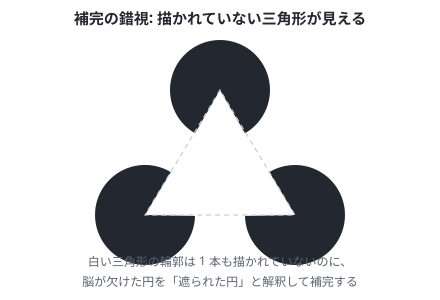
\includegraphics[width=0.85\textwidth]{figures/perception-fill.svg}
\caption{補完の錯視: 三角形は描かれていないのに見える}
\end{figure}

この仕組みは効率の源泉です。すべての情報を精密に処理していたら、脳の処理容量は足りません。\textbf{予測で穴を埋め、重要そうなものだけ精密に見る}。この経済的な設計が、時々あやまった見え方(錯視)を生む代償です。

\textbf{解答の指針:}\ 知覚の話を評するときは、「刺激(入力)」「処理(脳の解釈)」「見え方(知覚の結果)」の 3 段階に分けて書く。錯視は「刺激は同じなのに結果が違う」例で、処理の存在を証明する証拠です。「目が騙される」という表現ではなく「脳の解釈が見え方を作る」と書けるかが理解の目安です。

\section{記憶 — 3 つの貯蔵庫と忘却の法則}

記憶を「1 つの倉庫」と考えていると、現象が説明できません。実験が示すのは、\textbf{時間の枠と容量がまったく違う 3 つの貯蔵庫}が直列につながった構造です。

\subsection{感覚記憶・短期記憶・長期記憶}

\begin{itemize}
\item \textbf{感覚記憶}: 見たもの・聞いたものが数秒未満で消える受信バッファ。
\item \textbf{短期記憶(ワーキングメモリ)}: 今、頭の中で扱っている作業台。容量は約 4 つ分で、放置すると数十秒で消える。
\item \textbf{長期記憶}: 容量が事実上無限で、数日から一生残る倉庫。
\end{itemize}

\begin{figure}
\centering
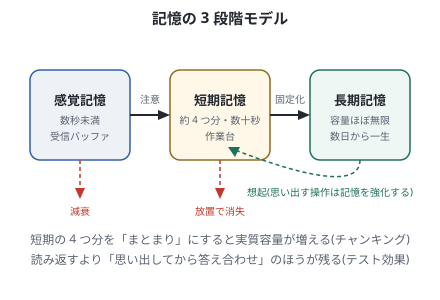
\includegraphics[width=0.9\textwidth]{figures/memory-model.svg}
\caption{記憶の 3 段階モデル: 保持と想起の流れ}
\end{figure}

短期から長期への移し替え(\textbf{固定化})には反復と意味づけが効きます。数字を 7 桁以上覚えにくいのは短期記憶の容量の限界であり、「3 つずつのまとまりに区切る」(電話番号の区切り)のが有効なのは、\textbf{1 つのまとまりを 1 項目として数えられる}からです。この操作を\textbf{チャンキング}と呼びます。

\subsection{忘却曲線と、思い出すことの効果}

エビングハウスの実験以来、\textbf{忘却は時間とともに急激に進み、やがて緩やかになる}ことが知られています(忘却曲線)。ここから得られる実用的な帰結は、\textbf{思い出すタイミングを忘れる直前に置くと効果が大きい}ということです。

さらに重要なのが\textbf{テスト効果}です。同じ時間を勉強に使うなら、「読み返す」より「思い出してから答え合わせ」のほうが、後の記憶の残り方が良い、という実験結果です。思い出す操作そのものが記憶を強化する。この本の図書館(テキスト・フラッシュカード・確認テスト)が復習を織り込んでいるのは、この知見が根拠です。

\begin{quote}
\textbf{【注意】}\ 記憶は録画ではありません。思い出すたびに内容が少しずつ再構成され、他の情報と混ざります。目撃証言の信頼性が議論されるのはこのためで、「記憶しているから正しい」は成り立ちません。
\end{quote}

\textbf{解答の指針:}\ 記憶の問題では、(1) どの貯蔵庫の話か(数秒なら感覚、数十秒なら短期、長期なら長期)、(2) 入力か保持か想起のどの工程か、を先に特定する。学習法を評する問題では、「思い出す操作が入っているか」「間隔が空いているか」の 2 点で判定します。読み返し中心の計画は、この 2 点で弱点を持っています。

\section{学習 — 条件づけと強化の仕組み}

「学習」は、心理学では\textbf{経験によって行動が変わること}と定義されます。知識の話ではなく、行動の変化の話です。2 つの古典的な実験系統があります。

\subsection{古典的条件づけ: 予告ができる}

パブロフの犬の実験は有名です。食べ物(無条件刺激)は自然に唾液を引き起こします。ベル(中性刺激)を食べ物の直前に鳴らし続けると、\textbf{ベルだけで唾液が出るようになる}。中性刺激が「食べ物の予告」を担うようになった、というのが\textbf{古典的条件づけ}です。

これは人間の日常にもそのまま当てはまります。歯医者の受付音で緊張する、特定の曲で昔の気持ちが戻る、などは予告学習の結果です。広告がブランドと良い気分を結びつけるのも同じ仕組みです。

\subsection{オペラント条件づけ: 結果が行動を形づくる}

スキナーの実験系統は、\textbf{行動の結果}が行動の頻度を変えることを示しました。\textbf{強化}(良い結果が続く)は行動を増やし、\textbf{罰}(悪い結果)は減らします。ただし罰は「何をしないか」しか教えられず、\textbf{代わりの正しい行動を教えない}弱点があります。教育の場で褒める(強化)中心が良いとされるのは、この理由です。

強化の\textbf{タイミングと頻度}も重要です。毎回報酬を与えるより、\textbf{まばらに与える}(間欠強化)ほうが行動が消えにくくなります。ギャンブルがやめにくいのは、まばらな大当たりが最も強力な間欠強化になっているからです。

\begin{quote}
\textbf{【注意】}\ 条件づけは「自動的な反応」の学習(古典的)と「自発的な行動」の学習(オペラント)で仕組みが違います。唾液や恐怖の反応は古典的、勉強を続ける習慣やゲームのプレイはオペラント。両方を混ぜて説明すると混乱します。
\end{quote}

\textbf{解答の指針:}\ 条件づけの問題では、(1) 刺激と反応の順番を書き出し、(2) ベル→唾液型の「予告」なら古典的、行動→結果型ならオペラント、と判定する。自分の習慣を分析するときは、「何が報酬として働いているか」「強化はまばらか毎回か」の 2 点を書き出すと、続かない理由が見えてきます。

\section{発達 — こころの成長の段階}

子どものこころは小さな大人ではありません。\textbf{思考の仕組みそのものが、段階を踏んで変わる}ことが発達研究の中心の発見です。

\subsection{ピアジェの段階と「保存の課題」}

ピアジェは、子どもに同じ量の水を細長いコップと太短いコップに移し替えて「どちらが多いか」を聞く実験(保存の課題)を行いました。ある時期までの子どもは、高さが上がったほうを「多い」と答えます。\textbf{見た目の変化と量の保存を、同時に考えられない}時期がある。これは頭が悪いのではなく、\textbf{論理の処理系がまだ構築途中}であることを示します。

成長は段階的に進み、感覚と動きで世界を掴む時期から、言葉とイメージの時期、論理的な操作ができる時期へと移行します。大切な帰結は、\textbf{教え方を相手の段階に合わせる必要がある}ことです。抽象的な説明が通じないのは、その段階の処理系では扱えないからです。

\subsection{愛着: 安全基地としての大人}

乳児と養育者の結びつき(\textbf{愛着})の研究では、養育者が安定した拠点(安全基地)になるほど、子どもは遠くまで探索し、新しい環境にも適応しやすくなる傾向が示されています。甘やかしと安全基地は別物で、\textbf{頼れる場所があるからこそ、チャレンジできる}という構造です。

\begin{quote}
\textbf{【注意】}\ 発達の段階は「何歳までに必ずできる」厳しいスケジュールではありません。個人差が大きく、平均からのずれは珍しいことではありません。段階の順序(先に何が、後に何が)のほうが、時期よりも堅実な知見です。
\end{quote}

\textbf{解答の指針:}\ 発達の話では、「その時期にできないのは、まだ処理系が整っていないから」という視点で書く。「教えれば分かるはず」「努力不足」と結論する前に、課題が相手の段階で処理可能かを確認する。保存の課題のような具体例を 1 つ持ち、「見た目の変化と、量や数の保存を同時に扱えるか」を軸に説明すると明快になります。

\section{社会心理 — 人は場に動かされる}

人間の判断は、個人の性格だけで決まりません。\textbf{同じ人が、場の構造だけでまったく違う行動を取る}。社会心理学は、この「場の力」を実験で測ってきました。

\subsection{同調: 全員が間違っていても}

アッシュの実験は、明らかに同じ長さの線分の比較問題を、被験者以外全員が意図的に間違えて答えるという設定でした。すると、\textbf{多数派に同調して明らかな誤答を繰り返す}被験者が一定の割合で現れました。視覚で確認できる事実ですら、場の圧力に屈する。ただし、答えを書く形式(他人が見えない)にすると同調は激減します。\textbf{屈していたのは視覚ではなく、目立ちたくない欲求}だったことが分かります。

\subsection{権威と役割: 靴白の服が持つ力}

ミルグラムの実験では、「学習者」に電気ショックを与える役を命じられた被験者が、白い服の実験者の「続けてください」という言葉に、苦痛の叫びを聞きながら指示に従う割合が高かった。権威とその場の設定(\textbf{役割})が、倫理観を上回る力を持つことを示した衝撃的な実験です(現在は倫理規定により同様の実験は制限されています)。

一方で、この実験は\textbf{権威への盲従を防ぐ教育}の重要性を示す知見でもあります。実験の参加者が、実験者に抗う口実(「医師の許可は?」)を与えられると従う割合が下がる、という追試もあります。\textbf{異議を唱えやすい仕組みを作ることが、盲従を減らす}のです。

\subsection{バイスタシー効果: 人数が多いほど助からない}

誰かが困っていても、周囲に人が多いほど誰も助けない(\textbf{バイスタシー効果})傾向が実験で示されています。理由は 2 つ。1 つは\textbf{責任の分散}(自分が助けなくても他の誰かがする)、もう 1 つは\textbf{多元的無知}(みんなが他人の反応を見て、困っていないと判断する)です。逆に、特定の個人に指名して頼む(「赤い服の方、救急車を呼んでください」)と、助かる確率が上がります。

\begin{quote}
\textbf{【注意】}\ これらの実験は「人間は悪い」の話ではありません。\textbf{場の構造が行動を決める}という話です。だから対策も、心がけ(個人の徳)ではなく、構造の変更(書記形式にする、指名する、異議を唱える口実を用意する)に置くのが正しい読み方です。
\end{quote}

\textbf{解答の指針:}\ 社会心理の問題では、(1) 「個人の性格」の説明と「場の構造」の説明を分けて書く、(2) 実験で場の構造をどう変えたか(他人が見えるか、責任が分散するか)を確認する、(3) 対策は構造の変更として述べる。この 3 段階で書けば、単なる啓発文ではなく社会心理学の答えになります。

\section{判断の近道 — ヒューリスティックとバイアス}

人間の判断は、毎回じっくり計算してはいません。\textbf{経験則(ヒューリスティック)で高速に答えを出し、時々系統的に間違える}(バイアス)。この研究は認知心理学と行動経済学の接点で、図書館の「行動経済学の落とし穴」と深くつながる分野です。

\subsection{2 つの近道: 使いやすさと引き金}

代表的な近道は 2 つです。

\begin{itemize}
\item \textbf{入手しやすさヒューリスティック}: 思い出しやすい例で確率を判断する。飛行機事故がニュースになるので、飛行機が危険だと感じるが、統計上は自動車より安全。
\item \textbf{代表性ヒューリスティック}: ステレオタイプに「似ているか」で確率を判断する。「無口で本が好き」と言われる人物を、司書か農家かで選ぶ問題で、司書を選びがちだが、実際は農家の母集団のほうがはるかに大きい(\textbf{基準率を無視する}誤り)。
\end{itemize}

近道自体は悪ではありません。\textbf{多くの場面で十分な答えを、少ない労力で出す}のが目的です。問題は、近道が系統的にずれる場面(確率・少数のサンプル・基準率が重要な場面)を知らずに使うことです。

\subsection{確率の場面でよく起こる誤り}

確率の場面で起きやすい誤りを 2 つ押さえます。

\begin{itemize}
\item \textbf{小数の法則の無視}: 小さなサンプルの偏りを、性質だと思い込む。「3 回連続で表が出たから次は裏」と考える(ギャンブラーの誤り)。
\item \textbf{確認バイアス}: 自分の仮説を支持する情報だけを集めて確認し、反する情報を見過ごす。
\end{itemize}

対策は、\textbf{近道を使っている自覚を持つこと}と、\textbf{反対の証拠を意図的に探すこと}です。判断の質は、頭の良さより手続き(どの証拠を見に行くか)で決まります。

\textbf{解答の指針:}\ 判断の誤りの問題では、(1) どの近道(入手しやすさか代表性か)を使っているかを特定し、(2) 本来使うべき数字(基準率・統計)を書き出し、(3) 2 つの答えの差を比べる。「なぜ間違えやすいか」を近道の効率で説明できれば、単なるリスト暗記から理解に変わります。

\section{感情とストレス — 仕組みと対処}

感情は「心の嵐」ではなく、\textbf{身体と連動した、測定可能な反応}です。測れるからこそ、対処も設計できます。

\subsection{闘争か逃走か: 身体の応答}

脅威を感じると、心拍・血圧・筋緊張が上がり、消化や免疫の一部は後回しになる。\textbf{闘争か逃走か}と呼ばれる身体の応答で、進化の産物として短期間なら有効です。問題は、\textbf{この応答が「実際の危険」と「心の中の危険(不安)」を区別できない}ことです。締め切りの不安でも、同じ身体反応が何日も続きます。

\textbf{ストレス}とは、この応答が長く続く(または反復される)状態です。ストレスの影響を測る研究から分かるのは、\textbf{出来事そのものより、出来事の主観的な評価と、制御感の有無}が負担を決めるということです。同じ負荷でも「自分で選んだもの」と「押しつけられたもの」では、身体の反応が違います。

\subsection{対処: 身体から入る方法}

対処の道具は 2 方向から入ります。1 つは\textbf{身体から}: 呼吸をゆっくり長くする(呼気を伸ばすと、興奮系のブレーキが入る)、運動で応答を消費してリセットする、睡眠で復元する。もう 1 つは\textbf{評価から}: 出来事の意味づけを変える(「脅威」を「挑戦」と再評価する)と、身体反応も変わることが実験で示されています。

\begin{quote}
\textbf{【注意】}\ 「ポジティブに考えろ」は対処法ではありません。評価の再構成は、出来事の現実を変えずに\textbf{対応の選択肢を増やす}操作です。現実を否定するのではなく、自分が制御できる部分を切り出して行動に移す、のが実用的な形です。
\end{quote}

\textbf{解答の指針:}\ ストレスの問題では、(1) 身体反応(心拍・ホルモン)の話と、(2) 評価(意味づけ)の話、(3) 制御感の話を分けて書く。対策を評するときは、「身体から入るか、評価から入るか、どちらの経路か」を明示する。睡眠・運動・呼吸が身体経路、計画と意味づけが評価経路の代表です。

\section{性格 — 型で語る危険と次元で測る方法}

「あの人は introvert(内向的)な性格」という言い方には、暗黙の仮定があります。\textbf{性格が型に分けられる}という仮定です。心理測定の研究は、この仮定に慎重です。

\subsection{型と次元の違い}

型の考え方(例えば 4 分割の性格分類)は、理解しやすい反面、\textbf{連続的な個人差を勝手に切り分けている}という問題があります。身長を「高い型・低い型」に分けるのが不自然なのと同じで、多くの心理的特性は\textbf{連続した次元}として測るほうが実態に合います。

現代の主流は\textbf{ビッグファイブ(BIG FIVE)}と呼ばれる 5 次元モデルです。

\begin{itemize}
\item \textbf{外向性}: 社交的で活発か、静かで内省的か。
\item \textbf{調和性}: 協力的で信頼するか、批判的で競争的か。
\item \textbf{誠実性}: 計画的で几帳面か、柔軟で即興か。
\item \textbf{神経症傾向}: 不安や気分の揺れを感じやすいか、安定しているか。
\item \textbf{開放性}: 新しい経験や考えを好むか、慣れたものを好むか。
\end{itemize}

\begin{figure}
\centering
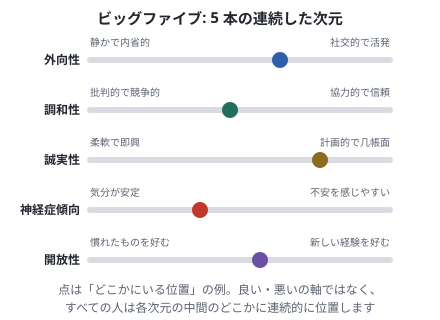
\includegraphics[width=0.9\textwidth]{figures/bigfive-dims.svg}
\caption{ビッグファイブ: 型ではなく 5 本の連続した次元}
\end{figure}

読み方の要点は 2 つ。\textbf{各次元に良い・悪いがないこと}、そして\textbf{人は各次元の中間のどこかに位置すること}です。誠実性が高いと計画は守れるが柔軟性は下がる、など、次元は特性の対応関係(トレードオフ)で読むのが正確です。

\subsection{性格と行動: 傾向はあるが決定ではない}

性格は行動の\textbf{傾向}を予測しますが、\textbf{場の構造}が強いときは性格が負けます(第 6 節の社会心理の知見)。性格と場の 2 要素で行動を説明するのが、現代の標準的な読み方です。「あの人はああいう性格だから」で説明を終える前に、場の構造を見直すほうが、行動の変化には効きます。

\textbf{解答の指針:}\ 性格の話では、(1) その説明が型か次元かを見分ける、(2) 次元なら「どの軸の、どの位置か」を書く、(3) 行動の説明に場の構造が含まれているかを確認する。4 分割などの型を批判するときは「連続量を切り分けている」「良い・悪いのラベルを生みやすい」の 2 点を挙げると整理できます。

\section{まとめと次の一歩}

9 節を振り返ります。道具は、実は 4 つしかありません。

\begin{itemize}
\item \textbf{実験の構造}: 何を測り、何と比べたか。結果より先に構造。
\item \textbf{3 つの貯蔵庫}: 記憶の流れ図。学習法のすべての根拠。
\item \textbf{条件づけ}: 予告の学習と結果の学習。習慣の設計図。
\item \textbf{場の力}: 同調・権威・責任の分散。個人の心がけより構造の変更。
\end{itemize}

心理学の学習で一番効くのは、\textbf{自分の日常を実験対象にすること}です。読んだ節について、自分の記憶の失敗・習慣の断続・判断の誤りを、この本の道具で書き直してみてください。心理学は「自分の心」を対象にできる数少ない科学で、道具を手にした瞬間から、観察が始められます。

次の一歩としては、この本の先は次のような本へつながります。

\begin{itemize}
\item 判断の誤りを経済の場面で → \textbf{行動経済学の落とし穴}(第 7 節の直接の続きです)
\item 学習の仕組みを勉強法に → \textbf{統計の勉強法}・\textbf{ノートと読み書きの技法}(第 3〜4 節の知見が根拠)
\item 記憶と判断をデータで守る → \textbf{統計学入門}(実験の結果の読み方の土台)
\item 心の働きを脳の物理で → \textbf{高校物理やり直し}(神経の電気信号の土台)
\end{itemize}

心理学は、測り方を学ぶことで初めて「心」を語れるようになる科目です。まずは身近な 1 つの習慣を、条件づけの道具で書き直すことから始めてください。

\end{document}
